\documentclass[11pt,a4paper,openany]{book}
% Preamble for the book. Serif text and maths, restrained colour.
\usepackage[utf8]{inputenc}
\usepackage[T1]{fontenc}
\usepackage{mathpazo}
\linespread{1.05}
\usepackage[a4paper,inner=30mm,outer=25mm,top=28mm,bottom=30mm]{geometry}
\usepackage{amsmath,amssymb,amsthm,mathtools}
\usepackage{booktabs,array}
\usepackage{graphicx}
\graphicspath{{../paper/diagrams/}{../paper/figures/}{figures/}}
\usepackage{caption}
\captionsetup{font=small,labelfont=sc}
\usepackage[expansion=false]{microtype}
\usepackage{xcolor}
\definecolor{rule}{gray}{0.55}
\usepackage[framemethod=default]{mdframed}
\newmdenv[linecolor=rule,linewidth=0.4pt,topline=true,bottomline=true,
  leftline=false,rightline=false,innertopmargin=6pt,innerbottommargin=6pt,
  skipabove=10pt,skipbelow=10pt]{practicebox}
\usepackage{natbib}
\usepackage[hidelinks]{hyperref}

\newcommand{\Prob}{\mathbb{P}}
\newcommand{\E}{\mathbb{E}}
\newcommand{\ind}[1]{\mathbf{1}\{#1\}}

\theoremstyle{plain}
\newtheorem{proposition}{Proposition}[chapter]
\newtheorem{corollary}[proposition]{Corollary}
\theoremstyle{definition}
\newtheorem{definition}[proposition]{Definition}
\newtheorem{assumption}{Assumption}[chapter]
\newtheorem{example}[proposition]{Example}
\theoremstyle{remark}
\newtheorem{remark}[proposition]{Remark}

% A short block for release committees at the end of a chapter's main text
\newenvironment{inpractice}[1][In practice]
  {\begin{practicebox}\noindent\textsc{#1}\par\smallskip\small}
  {\end{practicebox}}

% A planned chapter not yet drafted
\newcommand{\plannedchapter}[2]{\chapter{#1}\noindent\textit{Planned chapter, not yet drafted.}\par\medskip\noindent #2}


\title{Governing Disclosure Risk\\[6pt]
  \large Probability, Evidence and Accountable Decisions\\for Repeated Statistical Releases}
\author{Ronald Rethabile Malamule Mahomane}
\date{Working draft, November 2026. Not for circulation.}

\begin{document}
\frontmatter
\maketitle
\tableofcontents
\chapter{Preface}

This book grew out of a paper presented at the workshop on data security and
privacy that Banco de Portugal and the Irving Fisher Committee held in Lisbon in
September 2026. The paper argued that a disclosure risk figure only becomes useful
to an institution once it is attached to a declared attack, an honest statement of
its uncertainty and a written decision rule. In discussion, a participant asked
what happens to the risk when an institution gives several data sets to the same
researcher. The question went to the centre of the argument, and a conference
paper could only answer part of it. Chapter~\ref{ch:programmes} answers it in
full, and the rest of the book builds the framework that answer needs.

The book has two audiences, and it is arranged so that each can read it without
the other's material getting in the way. The first is the statistician, data
protection officer or release committee member at a central bank, statistical
office or health registry who has to decide whether a file goes out. For that
reader every chapter opens with the problem in institutional terms, states its
results in words before it states them in symbols, and closes its main text with a
short block headed \textit{In practice} that says what to write down and what to
check. The second audience is the researcher in statistics, computer science or
economics who wants to know exactly what is claimed and under which assumptions.
For that reader every result carries a numbered statement and a full proof, and
the proofs sit in a final section of each chapter so that the practitioner can
pass over them without losing the thread.

Every number in the book comes from one research pipeline, the Python
package \texttt{privacy\_risk} in the repository that accompanies the book. Where
a chapter reports a figure, it names the module and function that produced it, so
that a reader can rerun the calculation, change an assumption and see what moves.
Most of the evidence is synthetic. That is a limitation and the book says so
in the chapters it affects: the credit register in Part~V shares the structure of a
supervisory collection, but its parameters are chosen, not estimated, and the
floors it implies are conditional on that design.

The book also reports what did not work. The chapter on model-proposed attacks
includes a pilot in which augmenting the training data did not improve the model,
and the audit chapter shows how often an analyst who retries a failed audit
certifies an unsafe release. These results belong in the record because a method
for governing risk has to be judged on its failures as well as its successes.

This draft holds the preface, the first two chapters and Chapter~9. The other
chapters appear as short plans so that the reader can see where the argument goes.
Comments on the draft are welcome.


\mainmatter
\part{The problem}
\chapter{A risk figure is not a decision}\label{ch:decision}

Central banks, statistical offices and health registries release granular data
under a legal duty of confidentiality. The technical means of protecting those
releases are well developed. Cell suppression, minimum cell counts, global
recoding, record swapping, the cell-key method, added noise, synthetic data and
formal privacy mechanisms are documented, implemented in software and taught
\citep{willenborg2001,hundepool2012,dwork2014}. An institution that wants to
protect a file has no shortage of tools. What it usually lacks is a rule that turns
a measured risk into a decision to release or to withhold, a rule that someone
else could apply to the same evidence and reach the same answer.

This chapter sets out why that rule is missing, what goes wrong without it, and
what the rest of the book puts in its place.

\section{How release decisions are made now}

In most institutions the decision is made by committee. A disclosure control
officer presents a table of risk measures for the proposed release: perhaps the
share of sample-unique records, the smallest cell count, a mean re-identification
probability. A panel weighs those figures against the public value of the data,
and a decision follows. The decision is often sound, because the people on the
panel know the data and the users. It is rarely reproducible, however, and it is
hard to audit afterwards, because the quantity that decided the matter was never
written down. That quantity is the residual risk the institution was willing to
carry for this release, against this kind of harm, on someone's authority.

Better protection does not repair the gap. An institution can adopt a mechanism
with a formal guarantee, account carefully for its privacy loss parameter
$\varepsilon$, and still be unable to say what probability of harm it accepted,
because $\varepsilon$ bounds how far an adversary's beliefs can move rather than
how often an adversary succeeds (Chapter~10 returns to this). The same is true of
a minimum cell count. A floor of ten is a setting of the mechanism. It becomes a
statement about risk only under assumptions about the adversary that the floor
itself does not record, and Chapter~\ref{ch:scenario} shows how quickly those
assumptions fail.

\section{Three objects that are routinely run together}

The difficulty comes from treating three different objects as one. The first is a
probability model for an attempted linkage: given what a declared adversary knows
and what the release shows, how likely is it that the adversary names the right
record. The second is a statistical estimate of that probability, which in all
but the simplest cases comes from simulating the attack many times and so carries
sampling error. The third is a policy decision: how much residual risk is
acceptable, for which harm, on whose authority and until when.

The first is a modelling problem, the second an inference problem and the third a
governance problem. Each needs its own discipline, and running them together
produces failures that are easy to miss because each looks reasonable from inside
one of the three. Two examples show the pattern.

The first failure concerns the estimate. Suppose a committee releases a file
whenever the estimated risk falls below its tolerance. For a release whose true
risk sits exactly at the tolerance, a sensible estimator lands above and below the
true value about equally often, so the committee releases about half the time.
The committee believes it has a rule that keeps risk below the tolerance. It has a
coin toss at the boundary, and nothing in its records shows this, because the
records hold point estimates. Chapter~4 states this as a proposition and shows
that replacing the point estimate with a one-sided upper confidence bound
controls the chance of a wrong release at a stated level.

The second failure concerns the decision. An institution that says ``we apply a
minimum cell count of ten'' has stated a protection setting and called it a
policy. It has not stated the probability of harm it accepted, so nobody can check
whether the setting achieves the policy, and nobody owns the judgement that the
residual risk is acceptable. When the data change, or the users change, there is
no record of what the setting was meant to deliver, so there is nothing to
reassess against.

\section{What a decision rule needs}

The book's answer is a written decision rule with three parts, one for each of
the three objects. The model part declares an adversary: who attacks, what it
knows, which targets it attacks and what conditioning event the risk figure
assumes. The inference part replaces the point estimate with an upper confidence
bound at a stated error probability. The governance part states a tolerance and
attaches to it the things that turn a number into a decision: an owner
who accepts the residual risk, an expiry date, the harm class the tolerance is set
for, the legal basis and the parties it protects, the access route through which
the data will be used, and, for a series of releases, the horizon over which the
risk is assessed.

A release is then admissible when the upper bound for every target in a declared
target set lies at or below the tolerance. This is a simple rule, and its
simplicity is the point. Two analysts given the same declarations and the same
simulation output reach the same decision, and an auditor can check afterwards
that the decision followed from the evidence.

The rule has a price, and the book does not hide it. The evidence needed to
certify a tolerance grows as the tolerance shrinks. If an institution simulates an
attack many times and the attack never succeeds, the number of clean attempts
needed for a 95 per cent upper bound to reach a tolerance of one in a hundred is
299. For one in a thousand it is 2,995, and for one in a hundred thousand it is
299,572. Observing no successful attack never shows that the risk is zero, and
choosing a tolerance and choosing the evidence standard turn out to be one decision. Chapter~4 derives these figures and discusses what an institution
should do when the price is too high.

\section{Several releases from one register}

Single releases are not the operative problem. Institutions publish programmes: a
quarterly series, a research file and a public extract, all drawn from one
register. An adversary who holds several of these is not obliged to use them one at
a time. When records keep the same pseudonym across releases, the adversary can
intersect the candidate sets that each release leaves, and the result can identify
a target that no single release exposes.

The consequence is stronger than intuition suggests. Chapter~\ref{ch:programmes}
proves that no function of the per-release risks can bound the risk of an adversary
who pools the releases. Each release can be made as safe as one likes, judged on
its own, while the pooled releases identify the target with certainty. The
quantity an institution certifies when it reviews releases one by one is therefore
not the quantity that governs its exposure. On a simulated register, four releases
that each keep at least three records in every key class, and that contain no
unique record at all, identify the target with probability 0.458 once pooled,
against an upper bound of 0.253 implied by the four marginal risks. A quarter of
targets are identified uniquely by the intersection although none was unique in
any single release.

This is the question a workshop participant raised in Lisbon, and it is the reason
the book gives programmes a part of their own.

\section{A running example}

Most chapters return to one example: a synthetic credit register built to share
the structure of a supervisory collection such as the euro area's AnaCredit
\citep{israel2017}. It holds 20,000 firms as borrowers, 60 lenders with unequal
shares, 18 sectors, 12 regions and four size classes, observed over six monthly
vintages. About 27,000 loans are live at any time. Each released loan carries a
persistent pseudonym, its sector, region and size class, and its exposure.

The register is synthetic because real loan-level credit data are not released for
general use, and that choice limits what the example can show. Its parameters are
chosen by design, so the protection settings it implies describe the simulation
and not an actual institution. What the example can show is how the decision rule
behaves when the adversary changes. At an illustrative tolerance of 0.12, an
assessment of one release at a time passes the file with no suppression. An
adversary who pools the six vintages and knows in which of them the target's loan
was live requires a minimum cell count of 75. One who also holds a reading of the
loan's exposure in each vintage requires 150, and at that floor the file keeps 20
per cent of loans but only 4 per cent of exposure, with no loan to a large firm.
Against that adversary a loan-level file is the wrong product, and aggregates or
access in a secure setting are the realistic options. Part~V develops the example
in full.

\section{How the book is arranged}

Part~I sets up the problem. Chapter~\ref{ch:scenario} defines disclosure risk as
the outcome of a declared attack, derives the familiar reciprocal-frequency
measure from four assumptions and shows what happens when two of them fail.
Chapter~3 shows that the measures reported under one label answer different
questions. Part~II treats the risk figure as an estimate: its uncertainty, the
choice among protection settings, and certification while an attack is being
monitored. Part~III turns to the decision itself: the elements of a governance
threshold, and the tolerance implied by a stated weight on harm against utility.
Part~IV deals with programmes of releases and with formal privacy. Part~V reports
the evidence from simulation, public microdata, the credit register and a pipeline
in which a model proposes attacks. Part~VI is for practice: falsification tests, an
operational protocol and worksheets for six release types.

A reader who must decide on a release next month can read this chapter, the
\textit{In practice} blocks at the end of each chapter, and Part~VI. A reader who
wants to check the claims will find each one stated as a proposition with its
assumptions, and proved in the last section of its chapter.

\begin{inpractice}
Before the next release decision, write down four things that are usually left
implicit: the adversary the assessment assumes, the tolerance the release must
meet, the person who owns that tolerance, and the date after which the assessment
lapses. If any of the four cannot be written down, the committee is not yet in a
position to say whether the release is safe, whatever the risk table shows.
\end{inpractice}

\chapter{Disclosure risk as the outcome of a declared attack}\label{ch:scenario}

The minutes of the Bank's release committee contain one phrase more often than any other:
``every cell holds at least ten records, so no record carries a risk above one in ten.''
The chair wrote it, the committee approved it, and most readers of this book would approve it
too. It is the belief that a record's disclosure risk is the reciprocal of the number of
released records that share its key, so that a key class of ten means a one in ten chance.

The belief deserves its standing. The formula is old, it appears in every handbook, and it
answers a clear experiment: an adversary who knows a person's key, finds the released records
with that key, and picks one of them at random will be right one time in ten. The rule that
every class must hold at least $k$ records, known as $k$-anonymity, rests on it, and so do
most minimum cell counts in use at statistical institutions. If an adversary cannot tell the
records in a class apart, the formula is exact.

The fact that breaks it comes from a simulated register of 200,000 people with a 5 per cent
sample. A release that keeps at least ten records in every key class contains a record whose
own chance of being identified is 0.74, with a one-sided 95 per cent lower bound of 0.64.
% source: paper/generated/table_kanonymity.tex (k = 10 row: worst target 0.744, lower bound 0.638)
The adversary in that simulation knows one thing the key leaves out: a noisy reading of a
continuous variable that the release also publishes. That is enough to tell the ten records
apart.

This chapter asks one question: \emph{what does a disclosure risk figure measure, and under
what conditions does the reciprocal of the key frequency answer it?} The answer starts from
the objects every assessment involves, defines risk as the probability of one experiment, and
derives the familiar formula from that experiment under four assumptions. Stating the
assumptions shows where they fail, and two of them fail in the ordinary case.

\section{Population, sample, key and mechanism}

Let the finite population be $P = \{1,\dots,N\}$. The institution holds a
confidential sample, indexed by a random set $I \subseteq P$ of size $n$, and we
write $S_i = \ind{i \in I}$ for the inclusion indicator of unit $i$ and
$\pi_i = \Prob(S_i = 1)$ for its inclusion probability. A census is the case
$I = P$. Each unit has a confidential record $X_i$.

An adversary does not see all of $X_i$. It works through a key, a map $K_a$ from
records to a set of key values, where the subscript $a$ names the attack scenario.
The key collects the variables the adversary can observe about a person or firm
from outside: for a household survey perhaps age band, sex and district, for a
credit register perhaps sector, region and size class. For each key value $k$ the
population and sample frequencies are
\begin{equation}\label{eq:freq}
F_k = \sum_{i \in P} \ind{K_a(X_i) = k}, \qquad
f_k = \sum_{i \in P} S_i\, \ind{K_a(X_i) = k},
\end{equation}
so that $0 \le f_k \le F_k$. A record is sample unique when $f_k = 1$ and population
unique when $F_k = 1$.

The institution does not publish $X_I$ itself. It applies a protection mechanism,
which we write as a probability kernel $M_\theta$ indexed by a setting $\theta$, and
publishes a release $Y_\theta$ drawn from $M_\theta(\cdot \mid X_I)$. The notation
covers deterministic transformations, such as recoding or suppressing small cells,
as the case in which the kernel puts all its mass on one output. A minimum cell
count of five, a coarser age classification and a Laplace mechanism with
$\varepsilon = 1$ are all settings in this sense, and nothing so far requires a
setting to carry a formal guarantee.

Everything that follows depends on the randomness in the release, because a
disclosure risk is a probability over four sources at once: the sampling design,
the mechanism, the error in the adversary's own information, and any randomness in
the adversary's choice. An assessment that integrates over some of these and
conditions on others must say which, since the same file can give risk figures an
order of magnitude apart depending on that choice.

\section{One experiment}

Fix a target $t$ in the population. The adversary holds auxiliary information
$Z_t$ about the target, observes the release, and applies a linkage rule
$\delta_a$ that either names a released record as the target's or abstains.
Correct identification is the event that the target is in the file and the rule
names its record.

\begin{definition}[Scenario-conditional risk]\label{def:risk}
Given the background information $\mathcal{B}_a$ that scenario $a$ grants the
adversary, the unconditional and membership-conditional risks for target $t$ are
\begin{equation}\label{eq:tworisks}
R^{\mathrm{unc}}_a(t,\theta) = \Prob\{S_t = 1,\ \delta_a(Z_t,Y_\theta) = t \mid \mathcal{B}_a\},
\qquad
R^{\mathrm{in}}_a(t,\theta) = \Prob\{\delta_a(Z_t,Y_\theta) = t \mid S_t = 1,\ \mathcal{B}_a\}.
\end{equation}
\end{definition}

The two differ by the chance that the target is in the file at all. If a correct
link is impossible when the target is absent,
\begin{equation}\label{eq:factor}
R^{\mathrm{unc}}_a(t,\theta) = \pi_t\, R^{\mathrm{in}}_a(t,\theta).
\end{equation}
This is the multiplication rule of probability and involves no independence
assumption. It has practical weight because a sampling fraction is often applied
or omitted without comment, and with a 5 per cent sample that silent choice moves
the reported risk by a factor of twenty.

\section{Where the reciprocal of the key frequency comes from}

The most familiar disclosure measure assigns a record with key $k$ the risk
$1/f_k$: if three released records share the target's key, the adversary has a one
in three chance. The formula is usually presented as self-evident. It is in fact
the answer to the experiment above under four assumptions, which are worth stating
one by one.

\begin{assumption}\label{as:key}
The released key is unperturbed: applied to the release, the key map gives the
same values as applied to the confidential sample.
\end{assumption}
\begin{assumption}\label{as:obs}
The adversary observes the target's key without error.
\end{assumption}
\begin{assumption}\label{as:exch}
All records that share the target's key are exchangeable in the adversary's
information: nothing the adversary knows favours one of them over another.
\end{assumption}
\begin{assumption}\label{as:unif}
The adversary chooses uniformly among the records compatible with what it knows.
\end{assumption}

\begin{proposition}[Reciprocal frequency]\label{prop:recip}
Under Assumptions~\ref{as:key} to~\ref{as:unif}, for a target in the file whose key
is $k$,
\begin{equation}\label{eq:recip}
\Prob\{\delta_a = t \mid S_t = 1,\ K_a(X_t) = k,\ f_k\} = \frac{1}{f_k}.
\end{equation}
\end{proposition}

The result is old \citep{duncan1989,skinner2002}, and the value of restating it
lies in the list of conditions. Assumption~\ref{as:exch} fails whenever the
adversary holds a variable, correlated with something the release publishes, that
distinguishes candidates within a key class. In financial and health data that is
the normal case: a lender knows roughly how large its own loan to a firm is, and a
neighbour knows roughly how old someone is. Assumption~\ref{as:obs} fails whenever
the adversary's own source contains reporting error, which is also the normal case.
When either fails, the right object is no longer a frequency but a posterior
probability.

At the Bank this is where the chair's phrase runs into trouble. The credit register publishes
each loan's exposure beside its sector, region and size class. Pieter, a credit analyst at
one of the reporting lenders, knows the size of every loan his bank has made, give or take a
rounding. When he looks for one of his own borrowers in a class of ten, he does not choose at
random. He chooses the record whose exposure matches his books, and Assumption~\ref{as:exch}
no longer holds.

\section{When the assumptions fail}

Suppose the adversary's information and the released records are compared through
a likelihood, in the sense of record linkage under error \citep{fellegi1969}. Let
$L_{tj}$ be the likelihood of what the adversary observes under the hypothesis that
released record $j$ belongs to target $t$, let $q_{tj}$ be the prior weight on that
hypothesis, and let $j = 0$ stand for the hypothesis that the target is not in the
file. Bayes' rule gives the posterior
\begin{equation}\label{eq:post}
p_{tj} = \frac{q_{tj}L_{tj}}{q_{t0}L_{t0} + \sum_{\ell \in I} q_{t\ell}L_{t\ell}},
\end{equation}
and an adversary that names the most probable candidate succeeds with probability
\begin{equation}\label{eq:maxpost}
R^{\mathrm{in}}_a(t,\theta) = \E\Big[\max_{j \in I} p_{tj} \ \Big|\ S_t = 1,\ \mathcal{B}_a\Big].
\end{equation}
When the compatible records have equal likelihood and the no-match prior is zero,
\eqref{eq:post} and \eqref{eq:maxpost} reduce to the reciprocal frequency. In every
other case they can lie above or below it.

Two consequences follow, and both cut against common practice. First, measurement
error cannot be assumed to reduce risk. It changes the likelihood ratios, and it
may spread the posterior across candidates or concentrate it on one. In the
simulation study of Part~V, adding reporting error to the key lowers the
adversary's success from 0.466 to 0.381, while giving the adversary one noisy
reading of a continuous variable brings it back to 0.464. The reciprocal-frequency
figure was close to the truth in that case by cancellation, not by argument.

Second, a release can satisfy a minimum cell count on its declared key and still
expose individual records. If the release publishes a continuous variable, such as
an exposure or an income, and the adversary holds a noisy reading of it, the
posterior concentrates on the record whose value is nearest the reading, whatever
the size of the key class.

\section{$k$-anonymity is a threshold statement}

The rule that every released key class should contain at least $k$ records,
$k$-anonymity in the sense of \citet{sweeney2002}, is the most widely used
protection criterion in this field. The experiment above shows exactly what it
delivers.

\begin{proposition}[$k$-anonymity as a decision rule]\label{prop:kanon}
Under Assumptions~\ref{as:key} to~\ref{as:unif}, and for a tolerance
$\tau \in (0,1]$, the largest prosecutor risk in the release is at most $\tau$ if
and only if every occupied key class has at least $\lceil 1/\tau \rceil$ members:
\begin{equation}\label{eq:kanon}
\sup_{t \in I} \frac{1}{f_{K_a(X_t)}} \le \tau
\iff \min_{k:\,f_k>0} f_k \ge \lceil 1/\tau \rceil .
\end{equation}
If Assumption~\ref{as:exch} fails, for instance because the release publishes a
continuous variable of which the adversary holds a noisy reading, the implication
from right to left fails: there are releases that are $k$-anonymous on the declared
key in which some target's risk exceeds $1/k$.
\end{proposition}

Read this way, $k$-anonymity is a special case of the decision rule developed in
Part~III. It is the case in which the risk model is exact exchangeable matching,
the estimate carries no uncertainty, and the tolerance is the reciprocal of an
integer. Each of these simplifications is a place where an institution can be
wrong, and only the third is a policy choice. The failure in the second half of
the proposition is not hypothetical. On a simulated register of 200,000 units with
a 5 per cent sample, a release that is 10-anonymous on its declared key contains a
record whose own re-identification probability is 0.74, with a one-sided 95 per
cent lower bound of 0.64. Raising the minimum class size on that key does not
establish a bound for the enriched attack, because the variable that separates the
records is not part of the key.

The refinements of $k$-anonymity follow the same pattern. The $\ell$-diversity
criterion \citep{machanavajjhala2007} addresses the case in which all records in a
key class share a sensitive value, and $t$-closeness \citep{li2007} limits how far
the distribution of a sensitive value within a class may differ from its overall
distribution. Both protect against attribute disclosure, which can occur without
any record being identified. They change the risk model rather than the decision
rule, and they cannot be read as interchangeable tolerances for correct linkage.

Naledi ran Pieter's attack on the register before the next meeting. Against an adversary who
reads exposure with small error, the minimum cell count that the committee had treated as a
one in ten guarantee bounded nothing at all: Chapter~\ref{ch:credit} reports that no floor up
to 300 brings his success below the committee's tolerance. The chair's phrase was true of a
different adversary, one who knows only the key.

\section{What a risk figure must carry}

The argument of this chapter reduces to a requirement. A reported risk figure
should specify its scenario: who the adversary is, what it knows, which targets it
attacks, and which conditioning event the figure assumes, in particular whether the
target is known to be in the file. Chapter~3 shows that three measures commonly
reported under one label, all computed on the same simulated release, give 0.466,
0.064 and 0.023. Each is correct for its own experiment, and only a declared
scenario says which experiment the institution meant.

\section{The answer}

The question was what a disclosure risk figure measures and when the reciprocal of the key
frequency answers it. A risk figure measures the probability that a declared adversary, with
declared knowledge, names the right record in one defined experiment, and it means nothing
until that experiment is stated. The reciprocal of the key frequency is the exact answer when
the released key is unperturbed, the adversary observes it without error, nothing it knows
distinguishes the records in a class, and it chooses among them at random. When the adversary
holds a variable the release also publishes, or observes the key with error, the answer is a
posterior probability that can lie well above or below $1/f_k$, and a minimum cell count on
the key alone no longer bounds it. The chair's minutes should have read: ``no record carries a
risk above one in ten against an adversary who knows only the key.''

\begin{inpractice}
For every risk figure in a release assessment, record the adversary's auxiliary
variables and how precisely it observes them, whether the target is assumed to be
in the file, and whether the release publishes any variable outside the key that the
adversary might also know. If it does, a minimum cell count on the key alone does
not bound the risk, and the assessment needs a simulated attack that uses that
variable.

\smallskip\noindent\textit{In the software.} The measures of this chapter are in
\texttt{privacy\_risk.risk} (\texttt{prosecutor\_risk},
\texttt{marketer\_sample\_risk}, \texttt{marketer\_unconditional\_risk}), and the
posterior linkage of \eqref{eq:post} and \eqref{eq:maxpost} is in
\texttt{privacy\_risk.linkage} (\texttt{posterior\_linkage},
\texttt{maximum\_posterior\_success}, and \texttt{attack} for the simulated
version).
\end{inpractice}

\section{Proofs}

\begin{proof}[Proof of Proposition~\ref{prop:recip}]
Condition on $S_t = 1$ and $K_a(X_t) = k$. By Assumption~\ref{as:key} every
released record carries its confidential key, and by Assumption~\ref{as:obs} the
adversary observes $k$. The compatible set is therefore
$\{j \in I : K_a(X_j) = k\}$, which has $f_k$ members by \eqref{eq:freq} and
contains $t$. By Assumption~\ref{as:exch} the adversary's information is invariant
to permutations of that set, and by Assumption~\ref{as:unif} it selects each member
with probability $1/f_k$. Exactly one member is the target, so the probability of
a correct choice is $\sum_{j} f_k^{-1}\ind{j = t} = 1/f_k$.
\end{proof}

\begin{proof}[Proof of Proposition~\ref{prop:kanon}]
By Proposition~\ref{prop:recip}, the largest prosecutor risk in the release is
$1/\min_{k:\,f_k>0} f_k$. It is at most $\tau$ if and only if
$\min_k f_k \ge 1/\tau$, and since frequencies are integers this holds if and only
if $\min_k f_k \ge \lceil 1/\tau \rceil$, which is $k$-anonymity with
$k = \lceil 1/\tau \rceil$.

For the failure claim, drop Assumption~\ref{as:exch}. Let the release publish a
confidential variable $y$ beside the key, let a key class have exactly $k$ members
with distinct values of $y$, and let the adversary observe
$z_t = y_t + \sigma\xi$ with $\xi$ standard normal. Under the Gaussian likelihood
the posterior \eqref{eq:post} is largest for the member whose $y$ is nearest $z_t$.
Let $d > 0$ be the smallest gap between two values of $y$ in the class. The
maximum-posterior rule is correct whenever $|\sigma\xi| < d/2$, an event whose
probability tends to one as $\sigma \to 0$. Hence for all sufficiently small
$\sigma$ the target's risk exceeds $1/k$, while the release is $k$-anonymous on the
key for every $\sigma$.
\end{proof}

\plannedchapter{Measures that answer different questions}{The prosecutor, journalist and marketer measures computed on one release, why they differ by an order of magnitude, the sign of plug-in frequency bias, and the estimation of population uniqueness under a negative binomial frequency model.}

\part{Evidence}
\plannedchapter{A risk figure is an estimate}{Monte Carlo attack simulation, exact one-sided bounds, why a point estimate at the tolerance passes about half the time, the price of certifying small tolerances, and the split of variance between the simulation and the design.}
\plannedchapter{Choosing among protection settings}{Fixed-sequence testing from the most protective setting downwards, the independent confirmation draw, and why scanning a grid for any passing setting inflates false certification.}
\plannedchapter{Monitoring an attack while it runs}{Adaptive simulation budgets, the cost of retrying an audit, test martingales and confidence sequences that stay valid when the analyst looks at the results as they arrive.}

\part{Decisions}
\plannedchapter{Governance thresholds}{The nine elements of a threshold, the legal basis for central banks and data protection law, the protected parties of a credit register, the access route, and the separation of analyst, owner, reviewer and audit.}
\plannedchapter{Utility, harm and the tolerance they imply}{The risk--utility frontier, the tolerance a stated harm weight implies, why uniform tolerances across releases are usually inefficient, and how to allocate a programme tolerance as a risk budget.}

\part{Programmes}
\setcounter{chapter}{8}
\chapter{Several releases to the same user}\label{ch:programmes}

At the Lisbon workshop where this work was first presented, a participant asked
what happens to the risk when an institution gives several data sets to the same
researcher. The question is the right one to ask, because single releases are not
how institutions publish. A central bank releases a quarterly series, a research
file and a public extract, all drawn from one register, and a researcher with
access to one of them often has access to the others. This chapter shows that the
risk of the combination cannot be read off the risks of the parts, proves that no
rule based only on the parts can bound it, measures the gap on simulated and public
data, and sets out what an institution should assess instead.

\section{Two different questions about a programme}

Let an institution publish releases $Y_1,\dots,Y_m$. For each release let $C_i$ be
the event that the release, used on its own, allows a correct identification under
its declared attack, and let $R_i = \Prob(C_i)$ be its marginal risk. A natural
first question is the probability that at least one release, used alone, exposes
the target, which is the probability of the union
$C_\cup = C_1 \cup \dots \cup C_m$. The marginal risks say something about this
event, though less than one might hope.

\begin{proposition}[Sharp bounds from marginal risks]\label{prop:boole}
Without assumptions on how the events $C_i$ depend on one another,
\begin{equation}\label{eq:boole}
\max_i R_i \ \le\ \Prob(C_\cup)\ \le\ \min\Big(1,\ \sum_{i=1}^m R_i\Big),
\end{equation}
and both bounds are attained by suitable joint distributions, so the marginal risks
alone cannot identify a narrower interval.
\end{proposition}

The interval is wide. If the releases were independent, the union would have
probability $1 - \prod_i (1 - R_i)$, but releases cut from one register are
ordinarily dependent, since they describe the same people, and that expression
needs evidence before it can be used. In the simulation reported below the
independence value is 0.231 inside an interval of $[0.088, 0.253]$. It happens to
sit near the upper bound, and that agreement is a feature of the design and says
nothing about independence.

The second question is the one the participant asked, and it concerns a different
event. An adversary who holds all $m$ releases is not obliged to use them one at a
time. It can apply a joint linkage rule that looks at all the releases together, and
the programme risk is the probability $R_{\mathrm{pool}}$ that this joint rule names
the target. Success of the joint rule is not contained in the union of single-release
successes, so the bounds of Proposition~\ref{prop:boole} do not apply to it.

\section{Pooling intersects candidate sets}

Figure~\ref{fig:pool} shows the mechanism in its smallest form. Each of two
releases groups the target with two other records, so an adversary using either
release alone has a one in three chance. If both releases carry the same pseudonym
for each record, the adversary can keep only the records that appear in both
candidate sets, and here only the target does. Each release is as safe as a key
class of three makes it, and the pair identifies the target with certainty. The sum
of the marginal risks, two thirds, is no bound on the pooled risk.

\begin{figure}[ht]
\centering
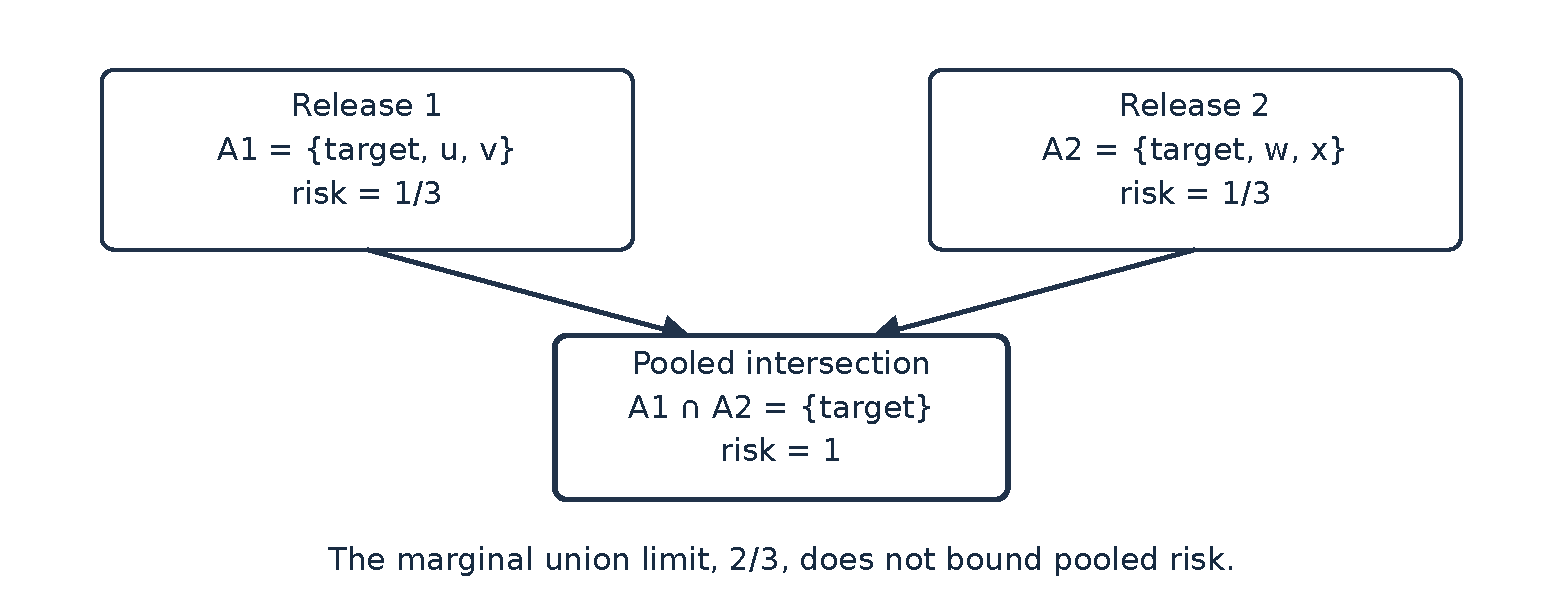
\includegraphics[width=0.78\textwidth]{pooling.pdf}
\caption{Pooling two releases intersects their candidate sets. Each release alone
leaves three candidates for the target; with a pseudonym common to both releases
the adversary keeps only records in both sets, which leaves one.}
\label{fig:pool}
\end{figure}

The small example generalises without limit, which is the central result of the
chapter.

\begin{proposition}[Marginal risks do not bound pooled risk]\label{prop:nopool}
Let $m \ge 2$. Suppose each released record carries a pseudonym that is the same in
every release, and the adversary knows the target's full set of quasi-identifiers,
from which it forms the target's key in every release. For every $\nu > 0$ there
exist a population, a sample and $m$ releases such that $R_i \le \nu$ for every $i$
while $R_{\mathrm{pool}} = 1$. Consequently no upper bound on $R_{\mathrm{pool}}$
can be written as a function of $(R_1,\dots,R_m)$ alone. If each release publishes
the candidate set implied by its key and the adversary chooses uniformly within the
intersection of those sets, then $R_{\mathrm{pool}}$ does not decrease as releases
are added, and $R_{\mathrm{pool}} \ge \max_i R_i$.
\end{proposition}

Neither the phenomenon nor its direction is new. \citet{sweeney2002} observed that
complementary releases, each $k$-anonymous, can be joined to re-identify;
differencing between linked tables is an old problem in disclosure control
\citep[ch.~4]{hundepool2012}; and \citet{ganta2008} showed that independent
releases of overlapping populations, each protected by a syntactic rule, can be
combined into a successful attack. Work on sequential releases of one table
\citep{wang2006,xiao2007} designs protection that survives republication. What the
proposition adds is a statement in the terms an institution uses when it certifies
a release: the quantity a programme is certified against, the per-release risk, is
not the quantity that governs it.

A persistent pseudonym also has a simpler reading. If every release carries the same
pseudonym, the adversary can join the releases into one table keyed on all the
variables any of them publishes. The pooled attack is then an attack on one release
with a finer key, and the proposition says that a finer key can carry far more risk
than any of its parts. That reading points to a remedy as well as a warning, and
Section~\ref{sec:prog-remedies} returns to it.

\section{How large the gap is}

Proposition~\ref{prop:nopool} is an existence result and says nothing about the
size of the gap in a real programme. To measure it, the pipeline draws four
releases from a simulated register of 200,000 units with a 5 per cent sample. Each
release is keyed on ordinary demographic variables, each keeps at least three
records in every key class, and none contains a single unique record. The four share
a record identifier.

Figure~\ref{fig:pool-sim} reports the result. The marginal risks lie between 0.017
and 0.088, so the marginals bound the chance that any one release succeeds between
0.088 and 0.253. An adversary who intersects only the first two releases already
succeeds with probability 0.411, which is 2.8 times the upper bound implied by those
two releases. With all four the pooled risk is 0.458, 1.8 times the bound implied by
all four. A quarter of targets, 26 per cent, are identified uniquely by the
intersection, although none was unique in any single release.

\begin{figure}[ht]
\centering
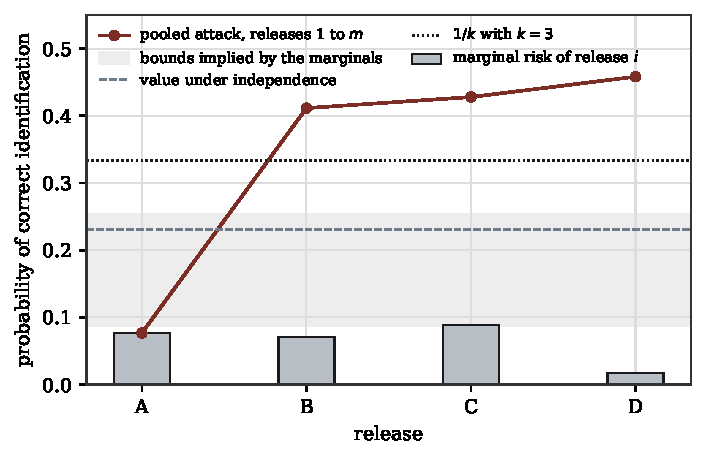
\includegraphics[width=0.8\textwidth]{fig4_composition.pdf}
\caption{Four 3-anonymous releases from one simulated sample: marginal risks, the
interval the marginals imply, and the risk of an adversary that pools releases 1 to
$m$, from 20,000 target replicates. Marginal risks are unconditional, so a target
suppressed from a release contributes zero to it.}
\label{fig:pool-sim}
\end{figure}

The gap is not an artefact of synthetic data. On a public file, an extract of the
US Census 2000 microdata, the same construction gives a pooled risk of 0.709 against
a bound of 0.381 from the marginals. Part~V reports both studies in full.

\section{The credit register}

The running example shows the same effect with an operational lever attached. The
synthetic register releases loans over six monthly vintages, each loan carrying a
persistent pseudonym, its borrower's sector, region and size class, and its
exposure. Judged one release at a time at a tolerance of 0.12, the file passes with
no suppression. The outcome changes once the adversary pools the vintages, but only
under a condition that is worth stating precisely.

\begin{proposition}[Without the history, the other vintages are uninformative]\label{prop:nohistory}
Suppose each loan's published key and exposure are the same in every vintage in
which it appears, that whether a loan is live in a vintage is drawn independently
of its key, its exposure and the adversary's auxiliary information, and that the
adversary knows only that the target is live in the first release. Then, for any
fixed auxiliary information, the adversary's posterior over candidates computed
from all vintages equals its posterior computed from the first vintage alone.
\end{proposition}

The result explains why pooling needs something extra to bite. Repeating the same
published fields adds nothing, and the pattern of months in which each loan is live
carries no information about which loan is the target unless the adversary knows
the target's own pattern. An adversary who does know in which vintages the target's
loan was live, as a counterparty or an informed observer might, can strike out every
candidate whose activity does not match. Against that adversary the decision rule
requires a minimum cell count of 75. An adversary who also holds a reading of the
loan's exposure in each vintage requires 150, and an insider who reads exposure with
small error is not stopped by any floor up to 300.

\section{What to assess instead}\label{sec:prog-remedies}

Three consequences follow for an institution that publishes programmes. First,
marginal risk figures may still be reported, because they describe what an
adversary achieves with one release, but they license no claim about the programme.
Second, a programme must be assessed by simulating the joint attack directly, with
targets and auxiliary information shared across the releases. Separate simulations
of each release cannot recover the dependence between them, because they never form
the intersection. Third, the programme needs a horizon: the number of releases over
which the joint risk is assessed, written into the governance threshold, with a
reassessment due before the next release beyond it. Pooled risk does not decrease as
releases are added, so a programme tolerance without a horizon has no fixed meaning.

The design of the identifier is the second lever. A pseudonym that persists across
releases is what allows the intersection, so rotating it between releases forces any
linkage to run through the published fields instead. The pseudonym itself should be
keyed, for example a keyed hash of the record identifier under a key held apart
from the release team, so that nobody can recompute it from the identifier.
Rotation is a control on linkability and not a guarantee. On the credit register it
does not help while exposure is published exactly, because the published key and
exposure relink every loan from one vintage to the next. With exposure rounded to
one significant figure they relink about one loan in ten. Whether rotation is worth
its cost therefore depends on what else the releases publish, and the joint
simulation is what tells the institution which case it is in.

A formal privacy accountant is the one device that composes across releases without
any assumption about how they depend on one another \citep{dwork2014}. Chapter~10
sets out what that guarantee says and what it leaves unsaid. A programme tolerance
can also be divided among releases as a budget on the union event, but by
Proposition~\ref{prop:nopool} such a budget governs the union only. It allocates
attention across releases and does not replace the joint simulation.

\begin{inpractice}[In practice: giving several files to one user]
List every release from the same register that the user can access, now and within
the assessment horizon, and every identifier or published field that could link
records across them. If records keep a pseudonym across releases, assess the pooled
attack directly by simulation rather than combining per-release figures. Record the
horizon in the decision record and set a reassessment before the first release
beyond it. If the pooled attack fails the tolerance at every acceptable floor,
consider rotating keyed pseudonyms, coarsening the linking fields, or moving the
user to a secure environment, and simulate again for each option.

\smallskip\noindent\textit{In the software.} The bounds and the pooled attack are
in \texttt{privacy\_risk.composition}: \texttt{marginal\_bounds} and
\texttt{independent\_union} for Proposition~\ref{prop:boole}, and
\texttt{pooled\_attack} (or \texttt{pooled\_attack\_from\_sets} for any release
format) for the intersection attack behind Figure~\ref{fig:pool-sim}.
\end{inpractice}

\section{Proofs}

\begin{proof}[Proof of Proposition~\ref{prop:boole}]
Each $C_i$ is contained in $C_\cup$, so $R_i \le \Prob(C_\cup)$ for every $i$, which
gives the lower bound. Subadditivity of probability gives
$\Prob(C_\cup) \le \sum_i R_i$, and $\Prob(C_\cup) \le 1$ always. For attainment of
the lower bound, let the events be nested, with every $C_i$ contained in the one of
largest probability; then $\Prob(C_\cup) = \max_i R_i$. For the upper bound, if
$\sum_i R_i \le 1$ let the events be pairwise disjoint, so that
$\Prob(C_\cup) = \sum_i R_i$; if $\sum_i R_i > 1$, place the events on a probability
space $[0,1)$ with Lebesgue measure as consecutive arcs of lengths $R_i$ wrapped
around the circle, so that together they cover the whole space and
$\Prob(C_\cup) = 1$.
\end{proof}

\begin{proof}[Proof of Proposition~\ref{prop:nopool}]
Fix $\nu > 0$ and choose an integer $k \ge 1/\nu$ with $k \ge 2$. Let the population
and the sample both consist of $k^m$ units, each labelled by a distinct vector
$(v_1,\dots,v_m) \in \{1,\dots,k\}^m$, and let these labels be the units'
quasi-identifiers. Release $i$ publishes every unit with its persistent pseudonym and
a key made of all coordinates except the $i$th. Units share a key in release $i$
exactly when they agree on every coordinate other than $i$, so every key class in
release $i$ has $k$ members, and under Proposition~\ref{prop:recip} of
Chapter~\ref{ch:scenario} the marginal risk of each release is $R_i = 1/k \le \nu$.

The adversary knows the target's label $(v_1,\dots,v_m)$, so in each release it can
find the target's key class and, through the pseudonyms, the corresponding set of
units. A unit in the class of release 1 agrees with the target on coordinates
$2,\dots,m$; a unit in the class of release 2 agrees with it on coordinate 1 and on
coordinates $3,\dots,m$. A unit in both classes therefore agrees with the target on
every coordinate, and since labels are distinct it is the target. The intersection of
the candidate sets is the target alone, so $R_{\mathrm{pool}} = 1$. Since $\nu$ was
arbitrary, any upper bound on $R_{\mathrm{pool}}$ written through the marginals
alone must equal one at marginals as small as we please, so no bound below one
exists.

For the last claim, let $A_i$ be the candidate set of release $i$, which contains the
target. The adversary's set after $j$ releases is $A_1 \cap \dots \cap A_j$, which
contains the target and shrinks as $j$ grows, so the uniform success probability
$1/|A_1 \cap \dots \cap A_j|$ does not decrease. Since the intersection of all the
sets is contained in each $A_i$, $1/|\bigcap_i A_i| \ge 1/|A_i| = R_i$ for every $i$,
and taking expectations over targets gives $R_{\mathrm{pool}} \ge \max_i R_i$.
\end{proof}

\begin{proof}[Proof of Proposition~\ref{prop:nohistory}]
Let $\mathcal{C}$ be the set of candidates the adversary forms from the first
vintage. For a candidate $j$, write $w_j$ for its published key and exposure and
$a_j$ for its pattern of activity across vintages. Under the hypothesis that $j$ is
the target, the joint probability of everything the adversary observes factorises
into a term for its auxiliary information given $w_j$, which is the term the first
vintage alone supplies, and a term for the activity patterns of all loans. The later
vintages contribute only copies of the $w_\ell$, which are already known from the
first, and the patterns $a_\ell$. Since activity is drawn independently of keys,
exposures and auxiliary information, and the adversary knows nothing of the target's
pattern beyond its presence in the first vintage, which every candidate shares, the
activity term is the same for every hypothesis $j \in \mathcal{C}$. It cancels from
the posterior, which therefore equals the posterior computed from the first vintage
alone.
\end{proof}

\plannedchapter{Formal privacy is a different regime}{What differential privacy bounds and what it does not name, the posterior an adversary may reach for a given $\varepsilon$, accounting across a programme, and how scenario assessment and formal accounting meet in one inequality.}

\part{Evidence from data}
\plannedchapter{A simulation study}{A synthetic population of 200,000 units with a 5 per cent sample: the measures side by side, the failure of $k$-anonymity under an enriched attack, and the cost of measurement error.}
\plannedchapter{Public microdata}{Two public files, including the US Census 2000 extract, the pooled attack on real keys, and what the public files can and cannot show about confidential registers.}
\plannedchapter{A granular credit register}{The synthetic register of 20,000 firms over six monthly vintages, the five harms, the floors each adversary requires, and what each floor keeps.}
\plannedchapter{Proposing attacks with a model}{The neural release pipeline and SENTRY-R: a model proposes scenarios and bets, a frozen plan records them, and an independent audit decides. The chapter reports the negative results alongside the positive ones.}

\part{Practice}
\plannedchapter{Testing the model behind the figure}{Six falsification tests, from linkage calibration to adversary stress, and why a failed test blocks the decision rather than adjusting the figure.}
\plannedchapter{An operational protocol}{Seven steps, the roles they need, a filled decision record for the credit register, and remedies when a release fails.}
\plannedchapter{Worksheets for six release types}{Starting declarations for the release types common in central banks, with blank worksheets.}
\plannedchapter{What remains open}{Real institutional registers, time-varying exposures, attack coverage, and the claims the method cannot make.}

\backmatter
\begin{thebibliography}{99}

\bibitem[Duncan and Lambert(1989)]{duncan1989}
Duncan, G T and D Lambert (1989): ``The risk of disclosure for microdata'', \emph{Journal of Business and Economic Statistics}, vol 7, no 2, pp 207--217.

\bibitem[Dwork and Roth(2014)]{dwork2014}
Dwork, C and A Roth (2014): ``The algorithmic foundations of differential privacy'', \emph{Foundations and Trends in Theoretical Computer Science}, vol 9, no 3--4, pp 211--407.

\bibitem[Fellegi and Sunter(1969)]{fellegi1969}
Fellegi, I P and A B Sunter (1969): ``A theory for record linkage'', \emph{Journal of the American Statistical Association}, vol 64, no 328, pp 1183--1210.

\bibitem[Ganta et~al.(2008)]{ganta2008}
Ganta, S R, S P Kasiviswanathan and A Smith (2008): ``Composition attacks and auxiliary information in data privacy'', in \emph{Proceedings of the 14th ACM SIGKDD International Conference on Knowledge Discovery and Data Mining}, pp 265--273, ACM, New York.

\bibitem[Hundepool et~al.(2012)]{hundepool2012}
Hundepool, A, J Domingo-Ferrer, L Franconi, S Giessing, E S Nordholt, K Spicer and P-P de~Wolf (2012): \emph{Statistical Disclosure Control}, Wiley, Chichester.

\bibitem[Isra\"el et~al.(2017)]{israel2017}
Isra\"el, J-M, V Damia, R Bonci and G Watfe (2017): ``The Analytical Credit Dataset: a magnifying glass for analysing credit in the euro area'', Occasional Paper Series, no 187, European Central Bank, Frankfurt am Main.

\bibitem[Li et~al.(2007)]{li2007}
Li, N, T Li and S Venkatasubramanian (2007): ``$t$-closeness: privacy beyond $k$-anonymity and $\ell$-diversity'', in \emph{Proceedings of the 23rd IEEE International Conference on Data Engineering}, pp 106--115.

\bibitem[Machanavajjhala et~al.(2007)]{machanavajjhala2007}
Machanavajjhala, A, D Kifer, J Gehrke and M Venkitasubramaniam (2007): ``$\ell$-diversity: privacy beyond $k$-anonymity'', \emph{ACM Transactions on Knowledge Discovery from Data}, vol 1, no 1, p 3.

\bibitem[Skinner and Elliot(2002)]{skinner2002}
Skinner, C J and M J Elliot (2002): ``A measure of disclosure risk for microdata'', \emph{Journal of the Royal Statistical Society, Series B}, vol 64, no 4, pp 855--867.

\bibitem[Sweeney(2002)]{sweeney2002}
Sweeney, L (2002): ``$k$-anonymity: a model for protecting privacy'', \emph{International Journal of Uncertainty, Fuzziness and Knowledge-Based Systems}, vol 10, no 5, pp 557--570.

\bibitem[Wang and Fung(2006)]{wang2006}
Wang, K and B C M Fung (2006): ``Anonymizing sequential releases'', in \emph{Proceedings of the 12th ACM SIGKDD International Conference on Knowledge Discovery and Data Mining}, pp 414--423, ACM, New York.

\bibitem[Willenborg and de~Waal(2001)]{willenborg2001}
Willenborg, L and T de~Waal (2001): \emph{Elements of Statistical Disclosure Control}, Springer, New York.

\bibitem[Xiao and Tao(2007)]{xiao2007}
Xiao, X and Y Tao (2007): ``$m$-invariance: towards privacy preserving re-publication of dynamic datasets'', in \emph{Proceedings of the 2007 ACM SIGMOD International Conference on Management of Data}, pp 689--700, ACM, New York.

\end{thebibliography}

\end{document}
